\chapter{Previous Work on Relationship Extraction}
In this chapter, we first introduce the most popular pre-trained models that are currently used in natural language processing (NLP). Then we discuss different metrics that are used on Relationship Extraction. Lastly, we describe previous work done on the topic of training models for the relationship extraction task.

\section{Deep NLP Models}
Lately, NLP tasks have been dominated by solutions using pre-trained deep neural models with the Transformer architecture. This section aims to roughly describe such a model to a reader familiar with the basics of neural networks. We introduce the two big concepts used in such models: the Transformer architecture and pre-training. Then we are able to explain how an actual modern NLP model looks and is trained. We choose the BERT model for this purpose since it is likely the best-known, and we also use it later in this thesis. 



\subsection{The Transformer Architecture}
Suppose that we aim to perform some NLP task, like translation, using deep neural networks. We want the network to read a sentence in language A and output a translation of the sentence in language B. If the model was just a sequence of densely connected layers (so-called feedforward neural network), it would be nearly naive to expect the model to function. There is no structure that would help with gathering information about the entire sentence, and there is also no intuitive place where we would expect the model to switch from one language to another. There is nothing ensuring that the translated sentence is good. Those arguments are vague but might provide some intuition.

The recurrent neural networks (RNN) were used in the past to help the network capture the entire sentence. The RNNs introduce a cell that is more complicated than a typical neuron (perceptron). This cell usually has internal memory and the ability to both add and forget information. In the network, this cell is then presented with a sequence of inputs. The cell then goes trough the sequence one by one and edits its internal state. If we feed it with words of a sentence, we might expect the internal memory to contain an abstract representation of the sentence. 

There are two main issues with RNNs. Working with RNNs is slow. We input the sentence \vuvozovkach{word by word}, so instead of one step per layer, we need $n$ steps for a sentence of length $n$. Moreover, especially if the sentence is long, it is difficult for the cells to remember the whole sentence and not just the later part. Both of these issues arise from the fact that input is fed into RNN cells sequentially. 

In \cite{vaswani2017attention}, the Transformer architecture is introduced. It builds on a so-called encoder-decoder architecture. In the translation task, we can roughly say, that the encoder would process the sentence in language A, the decoder an already predicted part of the translated sentence, and the network would predict the next word of the translated sentence.


The issue of the accumulation of the right information at the right place is addressed with an attention mechanism. Attention was used first in the RNN architecture. The traditional attention mechanism makes it possible to focus only on the important parts of the input sentence. For example, if we want to translate a specific word in a sentence, the network can learn that some parts of the input sentence are more important than others. Later, it was discovered, that a variant of the attention itself, called \textit{self-attention}, is powerful enough to make the sequentiality of the RNN cells unnecessary.

Self-attention was introduced in the Transformer architecture. Unlike the traditional attention, which is used to combine information from different layers (for example, it can transfer information from encoder to decoder), the self-attention usually works with inputs of the same layer as where it is applied. Self-attention attempts to add context information to the current embedding from the current embedding of the input sequence. For each input vector, we first compute three vectors: key, query and value. When computing self-attention for the $i$-th input, we compute the dot product of the $i$-th query vector with each key vector, we call the resulting numbers scores. The $j$-th score represents the distance of the $i$-the query and the $j$-the key vector. We then convert the scores to non-negative numbers that sum up to 1 and use those values to weight the value vectors (simply by multiplication). Lastly, we sum such weighted vectors to create the $i$-th output. We described the operations on vectors, but they can be rewritten for whole matrices, which makes them faster to compute. Precisely, let $Q$, $K$ and $V$ be matrices, where the $i$-th row is the $i$-the query, key and value vector. Then the attention can be computed as $Attention(Q,K,V) = softmax(\frac{QK^{T}}{\sqrt{d}})V$, where $d$ is the dimension of the key vectors.


\begin{figure}[h]\centering
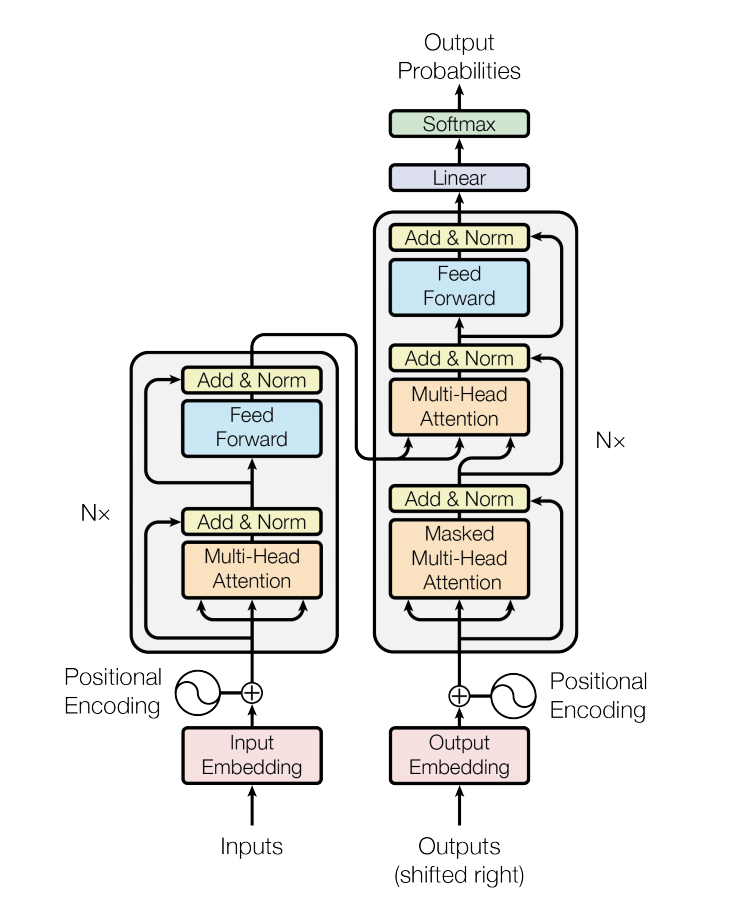
\includegraphics[scale=0.7]{./img/transformer}
\caption{Diagram of the Transformer architecture as proposed in \cite{vaswani2017attention}. Taken from \cite{vaswani2017attention}}
\label{obr:transformer}
\end{figure}


In the Transformer architecture, both the decoder and the encoder contain a sequence of blocks, where each block is a self-attention layer followed by a feed-forward network. We include a diagram of the architecture from the original paper (\autoref{obr:transformer})



So far, we ignored the fact that words cannot be directly fed to the network as an input. Usually, words are mapped to a vector in an embedding space. Such mapping is reusable in multiple tasks and brings us to the next section, where we will explain them a bit more.
 
\subsection{Pre-training}

The training of deep neural networks can require a great deal of both computational resources and annotated data. The term pre-trained model indicates a (part of) neural network, that can be reusable for multiple tasks or settings. Moreover, the pre-training is often based on unsupervised data, which lowers the requirements for annotated data later in the fine-tuning. Such reusability fastens deployment of complicated models and makes them accessible for a broader spectrum of people and companies. Pre-training is time-efficient, economical and consequently ecological.

Word embeddings can be seen as an example of pre-training. Word embedding is a vector that represents a word in a vector space (as, for models, vector spaces are easier to work with than words). The distance of embeddings of two words should reflect their semantic relation. An embedding itself is usually inferred from a pre-trained neural network and is used as an input for the task-specific model. The model that generates embeddings is usually trained by some variation of predicting a missing (masked) word from its context. The popularity of word embeddings rose in the previous years, most popular embeddings were likely the Word2vec \cite{mikolov2013word2vec}.  

Nowadays, a new type of embeddings is starting to get popular. In the classical word embeddings, a word always has the same embedding. The word \vuvozovkach{book} has the same embedding in \vuvozovkachtextit{She wrote a book on car maintenance.} and \vuvozovkachtextit{We were advised to book early if we wanted to get a room.} which is intuitively wrong. Contextualized embeddings take into account the entire (or at least preceding part of) sentence. One such embedding can be created via the BERT model.

\subsection{BERT}
\label{sec:bert}
BERT (Bidirectional Encoder Representations from Transformers, \cite{bert}) is a family of models that achieves state-of-the-art results on various NLP tasks. BERT model takes a sequence of words as an input and computes a representation of each word while taking into account both the left and right-side contexts of the word. BERT models are pre-trained on large corpora of unlabeled text and then fine-tuned for a specific task. 

The model was pretrained on two NLP tasks - Masked Language Modeling (MLM) and Next Sentence Prediction (NSP). 

MLM is an adaptation of the task of prediction of a word from its context. The model takes a sentence, where some percentage of the words is replaced with a special token. The goal is to predict the original words in the sentence. The masking is essential; without it, the task would be trivial; at the same time, some context has to stay unmasked; otherwise, the task would be impossible. If we always mask the percentage of the words with the special token, a significant mismatch between real sentences and the one used in training would be created. The masking is, therefore, more sophisticated. We choose 15\% of words to be masked. If a word is to be masked, with 80\% change, it is replaced with the special token, with 10\% it is replaced with a random word, and in the last 10\% the word is kept (which helps to bias the model towards the actual word).

In NSP, we try to guess whether two sentences were consequent in the original text. The input is structured into two sentences via a separator token and segment embeddings. This task helps the model to learn to work on the sentence level, not just on a token level.

To fine-tune the model, we usually add a shallow feed-forward network on top of the BERT, which classifies chosen features from the BERT into the result space. Then we train the model on the task-specific dataset as we would train any other model.

In the original paper (\cite{bert}) two BERT models were published: BERT\textsubscript{BASE} and BERT\textsubscript{LARGE}, they differ in size, but both trained on the same English corpora (the BookCorpus and English Wikipedia). Later multilingual BERT was released\footnote{\url{https://github.com/google-research/bert}}. It was trained on the top 100 languages with the largest Wikipedias.


\section{Metrics}
This section focuses on metrics since the quality of a model in the relationship extraction task is often hard to determine. We first define some standard metrics and discuss the pros and cons of each of them. Then we overview metrics used for the relationship extraction task on different datasets.

\subsection{Binary Classification}

We will start with metrics for binary classification. In binary classification, we are presented with an input vector, and the goal is to determine whether the vector is of class A for class B. Each prediction then falls into one of the following categories: correctly classified A input, correctly classified B input, wrongly classified A input as B, and a B input wrongly classified as A (Figure \ref{obr:CM}). 

\begin{figure}[h]\centering
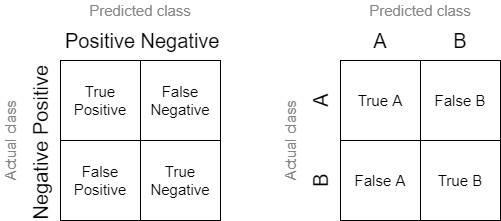
\includegraphics[width=0.9\textwidth]{./img//Diplomka diagramy-Confusion matric}
\caption{Confusion matrix for binary classification, normally count of occurrences would be written in each square. }
\label{obr:CM}
\end{figure}

Another way to look at the same situation is just to predict whether an input is of class A or not. This way the prediction is a True / False value determining whether the input is of class A. This way, we can define the previously mentioned categories without using the specific classes as \defineterm{true positive} (TP), \defineterm{true negative} (TN), \defineterm{false negative} (FN) and \defineterm{false positive} (FP). Visualization of the result of classification on a dataset is called a \defineterm{confusion matrix}, we include such matrix in \autoref{obr:CM}. We will use the abbreviations to represent the number of predictions that belong to the given category.  



\defineterm{Accuracy} expresses the ratio between correct predictions and all predictions.
\begin{align}
Acc = \frac{TP+TN}{TP+TN+FP+FN}
\end{align} 



\defineterm{Precision} expresses the ratio of correctly predicted positives within all predicted positives. Therefore, precision is a good metric if we want to avoid mistakenly classified negatives as positives.

\begin{align} 
Prec = \frac{TP}{TP + FP}
\end{align}

\defineterm{Recall} is the complementary metric to precision. It expresses the ratio of all positives that were correctly predicted. In other words, it should be used when we need to find the maximum of positives in the data.

\begin{align}
Rec = \frac{TP}{TP + FN}
\end{align}

Often we might want a trade-off between being as precise as possible and recalling as much as possible. \defineterm{F1 score} is a harmonic mean of precision and recall (scaled to range from 0 to 1): \begin{align}
F1 = 2\frac{Prec \cdot Rec}{Prec + Rec}
\end{align}
F1 is quite widely used in competition tasks.

%Let us show three use cases, each of the defined metrics will be the best fit in one case.

%Suppose we have a collection of pictures of cats and dogs for adoption. If we were to classify pictures of cats and dogs based on the animal, we would most likely want to maximize the number of correct predictions. Accuracy would aim exactly for that.

%If we knew that some adopters suffer from cynophobia (fear of dogs), suddenly the classifier should accommodate the fact by optimizing precision (where a cat is a positive). Note that precision (and recall) in binary classification will return different values if we swap which class is the positive and which is negative.

%If the demand for cats extends supply and therefore we have more dogs than cats in the collection, searching for cats could get harder. In such a case, we would want to make sure that all cats are actually classified as cats, and recall would help with that.


To emphasize that the right choice of metric is significant suppose that we have balanced data (both true and false classes are equally represented). If our classifier just predicted that every input is positive, we would obtain the following: 0.5 accuracy, 0.5 precision, and 1 recall. If we were to predict all negatives, accuracy and precision would remain 0.5 but recall suddenly drops to 0. If we were to predict the result with even chances for both classes randomly, the expected results would be 0.5 for all of those metrics. We just described three very different classifiers, and the only thing we learned from accuracy and precision was that they were equally bad, without any insight about them. Recall, in contrast, successfully gave us insight about what the predictions likely are, but evaluated a bad classifier with the highest possible score. We should also note, that the metrics will likely change if we exchange which class corresponds to True and which to False. 

This whole section is in this thesis mostly to remind us that if we want to score well in a given metric, we will likely exploit the metric even if it might worsen our classifier. The choice of a metric for a task determines what gets optimized. Later in this section, we will debate such issues in our scenario, in the relationship extraction task.





\subsection{Multiclass Classification}


We already run into issues with the asymmetry of precision and recall in binary classification (it is dependent on which class is chosen to be the positive one). We can address this by creating metrics per class. In the previous subsection, where we had a classifier for classes A and B, we would get two sets of metrics, each describing the ability of the classifier to recognize given class apart from the rest.

Now we can easily extend this per class approach to multiclass classification. The formulas will remain the same; only the way we obtain the TP, FP, TN, and FN values is a little different. In a sense, nothing changed - if we imagine that the classifier is still binary, then the situation is the same. However, if we compute those values out of confusion matrix (for class B) than TP is the value on position [B, B], FP is the sum of all in column B without TP, FN the sum of row B without TP and the sum of cells outside of the Bth row and column are the TN. (Figure \ref{obr:BigCM})



\begin{figure}[h]\centering
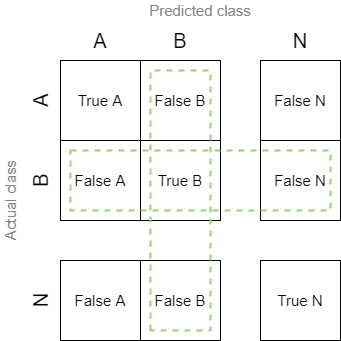
\includegraphics[width=80mm]{./img//Diplomka diagramy-Big Confusion matric}
\caption{Confusion matrix for N-class classification}
\label{obr:BigCM}
\end{figure}






As a robust way of examining the quality of the classifier, one could simply look at the confusion matrix and all the per-class metrics. Although this would be insightful, it is not the most practical in terms of a clear comparison of two classifiers. Ideally, we aim for a metric or metrics that are as descriptive and comprehensive as possible and also define an ordering of the classifiers.

Ideally, we would compute one number that fully describes the quality of the classifier. The common practice is to assign each metric a weight and combine them. Before we do so, we should acknowledge that the dataset we evaluate the classifier on needs to be taken into consideration.

An ideal dataset would be perfectly balanced. In real life, we encounter two types of imbalance in datasets:

\begin{itemize}
\item class representation distribution (CRD) is not uniform - classes are not equally represented 

\item class representation distribution is different in the test and the train part of the dataset
\end{itemize}
The second imbalance is tricky. Often, when optimizing the classifier, we do not know the CRD of the test dataset. We will, therefore, mostly focus on the first one. 


\subsubsection{Macro-averaged Metrics}

An easy way to combine a metric over multiple classes into a single value is to compute the arithmetic mean. In most libraries and papers, the term macro-[metric] (macro-recall, macro-F1, etc.) is used.  Macro averaged metrics tend to be the easy option that is used without much thought. So much so, that even though two different definitions of macro-F1s exist, the exact formula is often not included in papers. (The more common formula is the arithmetic mean of classes F1s, but the less commonly used formula where the F1 is computed from macro-recall and macro-precision is also used as  \cite{Opitz2019MacroFA} reports.)

\subsubsection{Micro-averaged Metrics}
The second most used approach of computing a single metric over multiple classes is to compute a weighted average with the weight corresponding to the support of individual classes. In most libraries and papers, the term micro-[metric] (micro-recall, micro-F1, etc.) is used. 

The main difference between micro and macro metrics is that macro metrics treat all classes equally, i.e. if there is a massively under-represented class, the metric prefers TODO. On the other hand, we should use a micro metric if we want to optimize the total accuracy of the model.

\subsection{Relationship Extraction Metrics}

In \nameref{chap:datasets} we described three relationship extraction datasets. In this subsection, we will focus on the metrics they use and propose the recommended metric for CEREDs.

\subsubsection{S10T8 metric}
For the S10T8 datasets, authors (\cite{semeval}) define the official metric directly in the paper: \vuvozovkach{Our official scoring metric is macro-averaged F1-Score for (9+1)-way classification, taking directionality into account.} This means that the model classifies into all $2*9+1$ classes, but before they compute the macro averaging, they merge the result into only the $9+1$ direction-less classes.

\subsubsection{TACRED}
On TACRED's git page\footnote{\url{https://github.com/yuhaozhang/tacred-relation}}, we can find the official implementation of an evaluator which computes a slightly modified version of micro metrics. Micro metrics are computed as the average of metric per class weighted by the support of that class. The authors modified the metric such that the weight of the \relationtype{no relation} class is zero. The micro-F1 is computed from the micro-precision and micro-recall. The primary metric for comparing results seems to be the micro-F1.

The decision to exclude the \relationtype{no relation} class is understandable. The class makes up 80\% of the dataset, therefore the micro metrics would be mostly influenced by the performance on this class. Such behaviour is unwanted considering the fact, that in usual use cases we care more about the model to correctly classify positive relations rather than the negative one. We would like to note that it is not possible to cheat the metric by forbidding the classifier to predict the negative relation. If we do so, it would negatively influence the false positives of all classes and, therefore, decrease the overall performance.


\subsubsection{Riedel NYT}

For the Riedel NYT dataset, there was no official metric determined by the authors. Papers report different metrics and therefore the results are hard to compare.


\subsubsection{CERED}

The Riedel NYT dataset shows, that we should decide, what the primary metric for CEREDs will be. We decided to use micro-F1. The negative relation in our datasets is not as dominant as in TACRED, so we do not think it is necessary to exclude it. On the other side, the datasets is not as nicely balanced as S10T8 and any macro-metric would be incline the models to overly focus on smaller classes.




\section{Relationship Extraction Models}

\chybi{matching the blanks .. psát? i když se neimplementuje? U výsledků je dvakrát zmiňuji, že jsou nejlepší}
\chybi{nebo tuhle sekci prostě odstranit?}


